\documentclass[a4paper,uplatex]{jsarticle}

\usepackage{iapaper}
\usepackage[dvipdfmx]{graphicx,xcolor}
\usepackage{listings}
\usepackage{amssymb}


\begin{document}
\pagenumbering{arabic} 

%New colors defined below
\definecolor{codegreen}{rgb}{0,0.6,0}
\definecolor{codegray}{rgb}{0.5,0.5,0.5}
\definecolor{codepurple}{rgb}{0.58,0,0.82}
\definecolor{backcolour}{rgb}{0.95,0.95,0.92}

% JavaScript
\lstdefinelanguage{JavaScript}{
  morekeywords={typeof, new, true, false, catch, function, return, null, catch, switch, var, if, in, while, do, else, case, break},
  morecomment=[s]{/*}{*/},
  morecomment=[l]//,
  morestring=[b]",
  morestring=[b]'
}

% CSS
\lstdefinelanguage{CSS}{
  keywords={color,background-image:,margin,padding,font,weight,display,position,top,left,right,bottom,list,style,border,size,white,space,min,width, transition:, transform:, transition-property, transition-duration, transition-timing-function},	
  sensitive=true,
  morecomment=[l]{//},
  morecomment=[s]{/*}{*/},
  morestring=[b]',
  morestring=[b]",
  alsoletter={:},
  alsodigit={-}
}

\lstdefinelanguage{HTML5}{
  language=html,
  sensitive=true,	
  alsoletter={<>=-},	
  morecomment=[s]{<!-}{-->},
  tag=[s],
  otherkeywords={
  % General
  >,
  % Standard tags
	<!DOCTYPE,
  </html, <html, <head, <title, </title, <style, </style, <link, </head, <meta, />,
	% body
	</body, <body,
	% Divs
	</div, <div, </div>, 
	% Paragraphs
	</p, <p, </p>,
	% scripts
	</script, <script,
  % More tags...
  <canvas, /canvas>, <svg, <rect, <animateTransform, </rect>, </svg>, <video, <source, <iframe, </iframe>, </video>, <image, </image>, <header, </header, <article, </article
  },
  ndkeywords={
  % General
  =,
  % HTML attributes
  charset=, src=, id=, width=, height=, style=, type=, rel=, href=,
  % SVG attributes
  fill=, attributeName=, begin=, dur=, from=, to=, poster=, controls=, x=, y=, repeatCount=, xlink:href=,
  % properties
  margin:, padding:, background-image:, border:, top:, left:, position:, width:, height:, margin-top:, margin-bottom:, font-size:, line-height:,
	% CSS3 properties
  transform:, -moz-transform:, -webkit-transform:,
  animation:, -webkit-animation:,
  transition:,  transition-duration:, transition-property:, transition-timing-function:,
  }
}

%Code listing style named "mystyle"
\lstdefinestyle{mystyle}{
  backgroundcolor=\color{backcolour}, commentstyle=\color{codegreen},
  keywordstyle=\color{magenta},
  numberstyle=\tiny\color{codegray},
  stringstyle=\color{codepurple},
  basicstyle=\ttfamily\footnotesize,
  breakatwhitespace=false,         
  breaklines=true,                 
  captionpos=b,                    
  keepspaces=true,                 
  numbers=left,                    
  numbersep=5pt,                  
  showspaces=false,                
  showstringspaces=false,
  showtabs=false,                  
  tabsize=2
}
\lstset{style=mystyle}

\title{レポート名}
\vspace{350pt}
\Yourname{Your Name}
\IDnumber{学生番号 Your Number}
\submissiondate{2024年1月31日}
\maketitle

\setcounter{page}{1} % 1から振り直す

\report{課題の概要}

\section{問題に関して}

\section{問題に関して}



% 箇条書き
% \begin{itemize}
% \item hoge
% \item foo
% \item bar
% \end{itemize}

% 箇条書き(番号付き)
% \begin{enumerate}
%     \item hoge
%     \item fuga
%     \item bar
% \end{enumerate}

% ソースコードの挿入
% 詳細: https://www.overleaf.com/learn/latex/Code_listing
% \begin{lstlisting}[language=Javascript, caption=p5.js start sample, label={list:label}]
% function setup() {
%   createCanvas(400, 400);
% }

% function draw() {
%   background(220);
% }
% \end{lstlisting}

% \subsection{図表の入れ方}
% 図\ref{fig:naist}のようにして記述すればok
% \begin{figure}[t]
%   \begin{center}
%     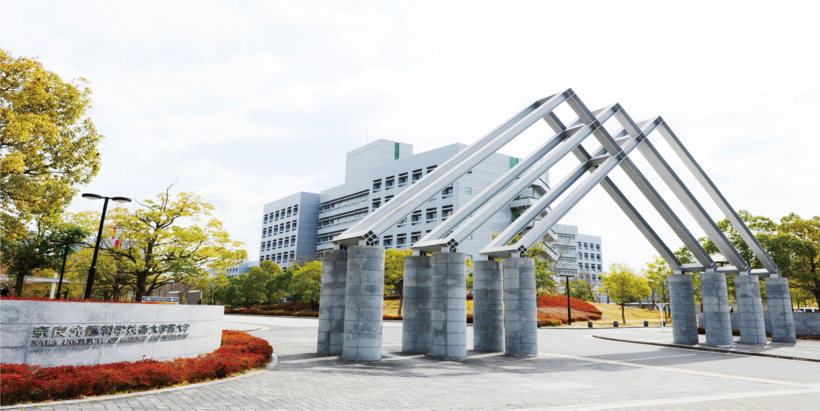
\includegraphics[width=0.95\hsize]{./images/sample.jpg}
%     \caption{NAIST}
%     \label{fig:naist}
%   \end{center}
% \end{figure}


%%% 参考文献をbibtex形式で引用する場合は上記の参考文献箇所はコメントアウトし、以下をコメントインする。
%%% junsrt: 引用順に文献番号を振る
%%% jplain: アルファベット順に文献番号を振る
\bibliographystyle{junsrt}
\bibliography{references}
\end{document}
